\chapter{Web Application Architecture}
\label{chap:webapparch}
This chapter describes the architecture of web applications. After an introduction to different web and web-related technologies and their roles, the differences between \emph{thin client} and \emph{rich client} web applications are discussed.
\section{Supporting Technologies}
The following section gives an overview of different technologies that are used in web applications (and other browser-based applications) nowadays. This list does not claim to be complete, but it covers those technologies important for the discussion.
\subsection{Server Side}
\begin{description}
	\item[\gls{http}] is the application layer network protocol of the web. \gls{http} is a textual, stateless protocol using \acs{tcp}. In a web environment, a web server --- such as Apache, Lighttpd, or Microsoft \gls{iis} --- acts as the \gls{http} server, whereas a web browser usually acts as the \gls{http} client. Not only web pages are transferred using \gls{http}, but also resources like \ac{css}, scripts (e.g. JavaScript files), \gls{xml} data and images. \gls{http} is an open standard developed by the \gls{ietf} and the \gls{w3c}.
	\item[HTML Preprocessors] are compilers or interpreters that generate \gls{html}. Some programming languages are especially built for this purpose, but in general, every programming language and compiler can be used to generate \gls{html}. Some of these preprocessors, such as \acs{php}, Perl and Python, are invoked through the \gls{cgi} of web servers. Others are used with application servers instead, for example \gls{asp}, ASP.NET, and \gls{jsp}. In the area of enterprise applications, \gls{jsp} has become the established standard.

	HTML preprocessors allow the dynamic generation of HTML, XML and other resources through the use of --- mostly imperative --- programming languages. The power of functions, variables and \glspl{api} can be used, for example to query a database and process the received data. This allows to overcome the statelessness of \gls{http}.
	\item[Application Servers] provide commonly used \glspl{api} and frameworks to applications, enabling them to use features such as security, load balancing, database connections or \gls{mvc}. Application servers are often used for enterprise applications, as they can shorten development time significantly. The most popular examples, such as Red Hat JBoss, Apache Tomcat, or IBM \gls{was}, can deploy Java and \acs{jee} applications, but there also are application servers for other programming languages, such as Zope for Python and Zend Server for \gls{php}. Usually, application servers include an \gls{http} server for the communication with web browsers, but this task can also be handled by a third-party web server.

	\gls{jee} application servers provide a \gls{jre} and consist of multiple components, including the following:
	\begin{itemize}
		\item The \emph{Servlet container}, also called \emph{web container}, manages \emph{Servlets} and maps them to a \gls{url}. A Servlet is a Java class that serves a client request with a special response, most often via \gls{http}. In other words, the Servlet container is the application server's interface to the web browser.
		\item The \emph{\gls{jsp} container} translates \gls{jsp} files into Servlets at runtime. \gls{jsp} features a templating system for \gls{html} that allows developers to embed Java code into \gls{html}.
		\item The \emph{\acs{ejb} container} manages \emph{\gls{ejb}}, which are components that encapsulate business logic in \gls{jee} applications. EJBs run back-end code and execute tasks like database access, messaging and web service invocation.
	\end{itemize}
	There are more components in the \gls{jee} specification, but they are not relevant in this context.
\end{description}
\subsection{Client Side}
\begin{description}
	\item[\gls{html}] is a markup language to represent hypertext\footnote{Hypertext resembles the thinking of human beings, in opposition to sequential text. Hypertext contains semantics and links to other texts, and is therefore non-linear.}. It was created by Tim Berners-Lee, who also developed the first web browser. \gls{html} consists of elements described by \emph{tags} which are enclosed by angle brackets. Tags often give semantics to elements, such as headings, emphasized text, lists or tables. Web browsers build a \gls{dom} out of \gls{html} code and display it as a web page.
	\item[CSS3] \gls{css} is a W3C standardized language to describe the look (``style'') of markup elements. It can be used, for example, to format and style an HTML document. The third generation of CSS adds more possibilities for designing user interfaces for web applications. In the past, visual enhancements such as shadows, gradients or non-standard fonts had to be provided by image files, and animations had to be programmed using JavaScript. CSS3 is capable of doing most of that while using less bandwidth and ensuring standards conformity, thus enhancing the performance and usability of websites. Some modern browsers even use hardware acceleration for CSS3 animations and effects. CSS3 makes complex user interface design possible on the web while separating the presentation from the content.

	In combination with CSS preprocessors\footnote{CSS preprocessors allow the creation of CSS from more versatile and powerful languages that are especially designed for this reason. Those languages, such as SASS, LESS, or Stylus, provide advanced features known from imperative languages, like variables and functions.}, such as SASS, LESS, or Stylus, development time can be reduced significantly.
	\item[JavaScript] is, according to \citeasnoun[p. 1]{flanagan}, ``the programming language of the web.'' It is a weakly~typed multi-paradigm language (functional and object-oriented), created 1995 by Brendan Eich at Netscape \cite{eich}. It is standardized as \emph{ECMAScript}, the latest version being ECMAScript 5.

	Most modern web browsers, such as Mozilla Firefox, Google Chrome, Opera or Microsoft Internet Explorer 9, provide a JavaScript engine and thus are able to execute JavaScript. Although they are not part of the language itself, \glspl{api} are provided by browsers to manipulate the \gls{dom} and use other browser functions, such as the browsing history. An event--callback system offered by the browser \gls{api} allows developers to build interactive web sites, in opposition to static ones based solely on \gls{html}. Different libraries and frameworks, such as Dojo, jQuery or Prototype, exist to simplify web application development with JavaScript.

	There are also server-side implementations --- for example \emph{Node.js}, which is based on Google's V8 JavaScript engine --- but they are not relevant in this context.
	\item[\gls{ajax}] is not a technology, but a method to allow dynamic loading of content, even after the actual web page has completely loaded. Using \pathname{XmlHttpRequest}, an object provided by the browser, HTTP requests can be sent from within JavaScript. The response, once returned, can then be processed in the background. The request is asynchronous, which means that the web page is not blocked while waiting for the response; it continues reacting to user input. This is especially important if the web page should feel like a desktop application.

	The method is called \acl{ajax}, because the response format often is \gls{xml}. However, this does not need to be the case. The response can be of any kind, for example an image, \gls{html} or \gls{json} data. \gls{json} is a subset of the JavaScript language, which means it can directly be included into the running script. Literals, objects and arrays can all be serialized as \gls{json}. In comparison to \gls{xml}, \gls{json} has a small footprint and a more flexible structure. The latter can, but not must, be a disadvantage.

	\item[HTML5] is the latest version of \gls{html}, which defines new elements and additional JavaScript \glspl{api}. Some of these \glspl{api} can be an advantage for MVC-based web applications, including:
	\begin{itemize}
		\item The \emph{Web Workers \gls{api}} relaxes the single-threaded client-side JavaScript model to support multiple threads, called ``workers''. Workers are to classic operation system threads; they do not share memory (thus, they lack access to the \gls{dom}) and can only communicate with the main thread through asynchronous messaging~\cite[pp. 680--687]{flanagan}. Nevertheless, Workers make it possible to execute multiple tasks in parallel without blocking each other or the user.

		\item Using the \emph{WebSocket \gls{api}}, long-living \acs{tcp} connections can be established. When using \gls{ajax} to communicate over the network, \gls{http} is always involved, which is a stateless (session--less) protocol. Opposed to that, WebSocket connections can be persistent and allow data to be sent and received as long as the socket is open. As WebSockets bring their own protocol on top of the \gls{tcp}, the server being queried also needs to support that protocol. There exist several libraries to add support to web servers, for example an Apache and a Node.js module \cite[pp. 712--716]{flanagan}.

		When used together with Web Workers, WebSockets can provide a web application with threaded network functionality. This is also relevant for MVC applications with real-time Model synchronization, as WebSockets can be used to notify the client of an updated server-side Model. This is further discussed in Section~\ref{sec:realtime}.

		\item The client-side \emph{Storage \glspl{api}} allow an application to store structured data within the web browser's sandbox. Before, only \gls{http} Cookies could be employed for client-side data storage, but Cookies are limited in size and they allow only textual data to be included. One of the new \glspl{api} is \emph{IndexedDB}, an object database that is currently supported in Firefox and Chrome, whereas the relational \emph{Web SQL} database is implemented in Chrome, Safari and Opera. The \emph{Filesystem API} allows web applications to create, delete and manipulate files and directory structures in a sandboxed environment. All web applications with the same origin (host, port, and protocol) share one filesystem --- this is a concept borrowed from HTTP cookies to avoid unauthorized access to data from the wrong web application.~\cite[pp. 700--712]{flanagan}

		These \glspl{api} can be used to allow advanced storage of data, breaking with the 4KiB limitation of \ac{http} cookies. They can be used for caching and client-side persistent storage. It is even possible to write offline applications using these APIs.
	\end{itemize}
\end{description}

\section{Client--Server Architecture on the Web}
\label{sec:clientserver}
This section describes the general architecture of 2--tier web applications, and then discusses the terms ``Thin Client'' and ``Rich Client'' in this context.

The first tier, also called ``client'', is the end user's web browser. The second tier, the ``server'', is a web server on the internet or inside a local network, for example a company's intranet. The key technology for this architecture is the \acs{http} protocol that has to be understood by both client and server. Thus, the web browser acts as an \acs{http} client and the web server acts as an \acs{http} server.

The common interaction between the user, a client and server using HTTP is further described by the following sequence diagram in Figure~\ref{fig:http}

\begin{figure}[H]
	\centering
	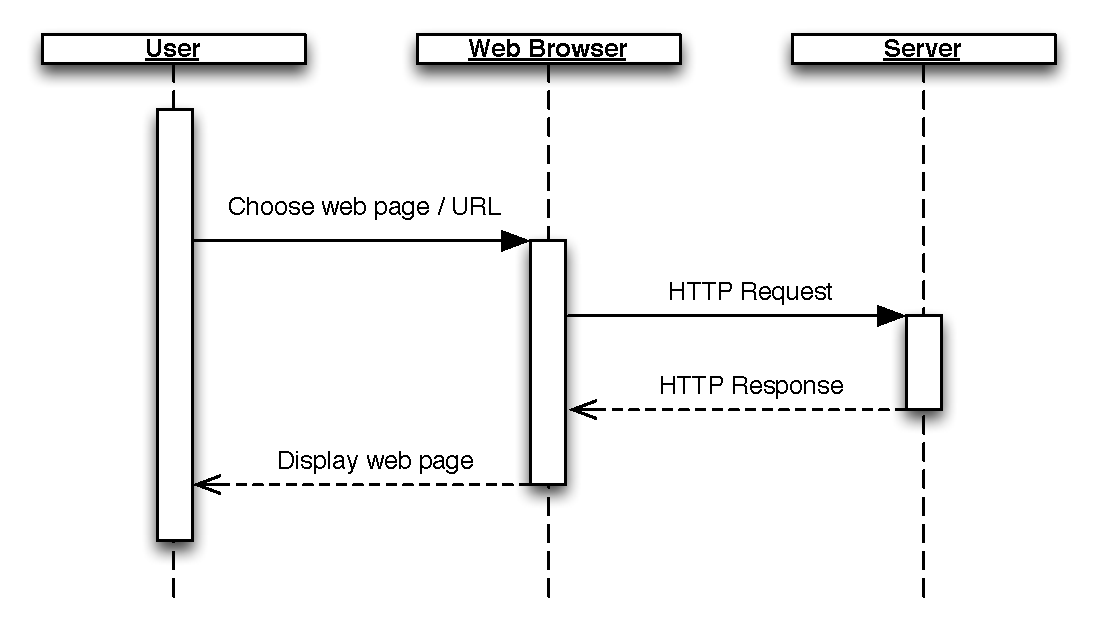
\includegraphics[width=16cm]{images/http.pdf}
	\caption{Sequence diagram of a User--Client--Server interaction}
	\label{fig:http}
\end{figure}

The actual HTTP request is illustrated in Listing~\ref{lst:http}. Such requests have to be made for every resource loaded from the server, such as \gls{html}, JavaScript, images and stylesheets (\gls{css}). As every request includes protocol overhead, the number of requests to be made is an important factor to the performance of a web application. This is further discussed in Section~\ref{sec:datavolume} and Section~\ref{sec:mvcwebarch}.
\begin{listing}[H]
\begin{minted}[linenos=true]{http}
GET /index.html HTTP/1.1
Host: www.example.com

HTTP/1.1 200 OK
Date: Mon, 23 May 2005 22:38:34 GMT
Server: Apache/1.3.3.7 (Unix) (Red-Hat/Linux)
Last-Modified: Wed, 08 Jan 2003 23:11:55 GMT
Content-Length: 438
Content-Type: text/html; charset=UTF-8

... Response body ...
\end{minted}
\caption{HTTP conversation}
\label{lst:http}
\footnotesize{\textbf{\textit{Source: \citeasnoun{wiki:http}}, modified by the author}}
\end{listing}
%Etag: "3f80f-1b6-3e1cb03b"
%Accept-Ranges:  none
%Connection: close

\subsection{Terminology}
\label{sec:terminology}
In computer technology, the terms ``Thin Client'' and ``Rich Client'' (also: ``Thick Client'' or ``Fat Client'') have multiple meanings, so it is necessary to define their meanings in this context.

These two terms often describe computer hardware. A Thin Client in the hardware context is a computer that heavily depends on another computer (e.g. a server) to fulfill its computational role, whereas a Rich Client not only handles input and output (I/O), but also processes data.

This concept of dependance also applies to web applications. In that context, the Thin and Rich Client are not computer hardware, but rather represent the client side of a web application (thus, they are software running \emph{inside a browser}).

The term ``Rich Internet Application'' also is sometimes used for web applications with a Rich Client, but it more often refers to applications powered by browser plug-ins, such as Adobe Flash or Adobe Flex.

The following two definitions are kept generic and reflect the fact that there are different variations in the range from a Thin to a Rich Client. Four of those variations are further discussed in Section~\ref{sec:mvcwebarch} with respect to an \ac{mvc} architecture. Both definitions are examined from both a user and technology perspective.

\subsection{Thin Client}
\label{sec:thinclient}
We can also refer to the Thin Client as the classical way of writing web applications. From a user perspective, a Thin Client feels like a usual web site. Every time the user switches the perspective or navigates to a different part of the web site, the \gls{url} changes and a whole page is loaded from the server. This is, for example, the fact with \url{http://www.craigslist.com/}\footnote{Craigslist is a classifieds platform extremely popular in the United States.}. If you switch between categories at the Craigslist web site, the whole page gets loaded and rendered again.

This is due to the fact that in many Thin Clients, every page of a web site either has its own \gls{html} file, or gets preprocessed on the server (using \gls{php}, \gls{asp}, \gls{jsp} or any other preprocessor) depending on defined parameters\footnote{These parameters may, for instance, be GET or POST parameters of the respective \gls{http} request \cite**{http}.}. From a technology perspective, a page is --- when requested --- constructed on the server side and sent over to the client side. There are no subsequent data loaded (except for resources already specified in the original page). The page is dynamically generated, but the web application is not interactive.

From the perspective of software architecture, a Thin Client is static and ``dumb''. Most of the business logic and data --- and thus, most of the \ac{mvc} structure if this is the used architectural pattern --- is on the server. The content gets prepared on the server, processed with real data and is then sent to the client. However, the client does not know where the data are from and how to retrieve additional or updated data. Also, it is not able to further process the data without communicating with the server. This means that a user can modify data on the client side, but these data must be sent back to the server side to be processed and then the updated page has to be retrieved again.

The sequence diagram (Figure~\ref{fig:seqthinclient}) shows the process of a user requesting a web page and then updating data using a Thin Client / Rich Server with an additional database tier. Business logic, for example input verification, is executed on the server. After updating the data, the whole web page has to be preprocessed on the server, sent to the client and displayed again. The browser and user are inactive during this time.

\begin{figure}[H]
	\centering
	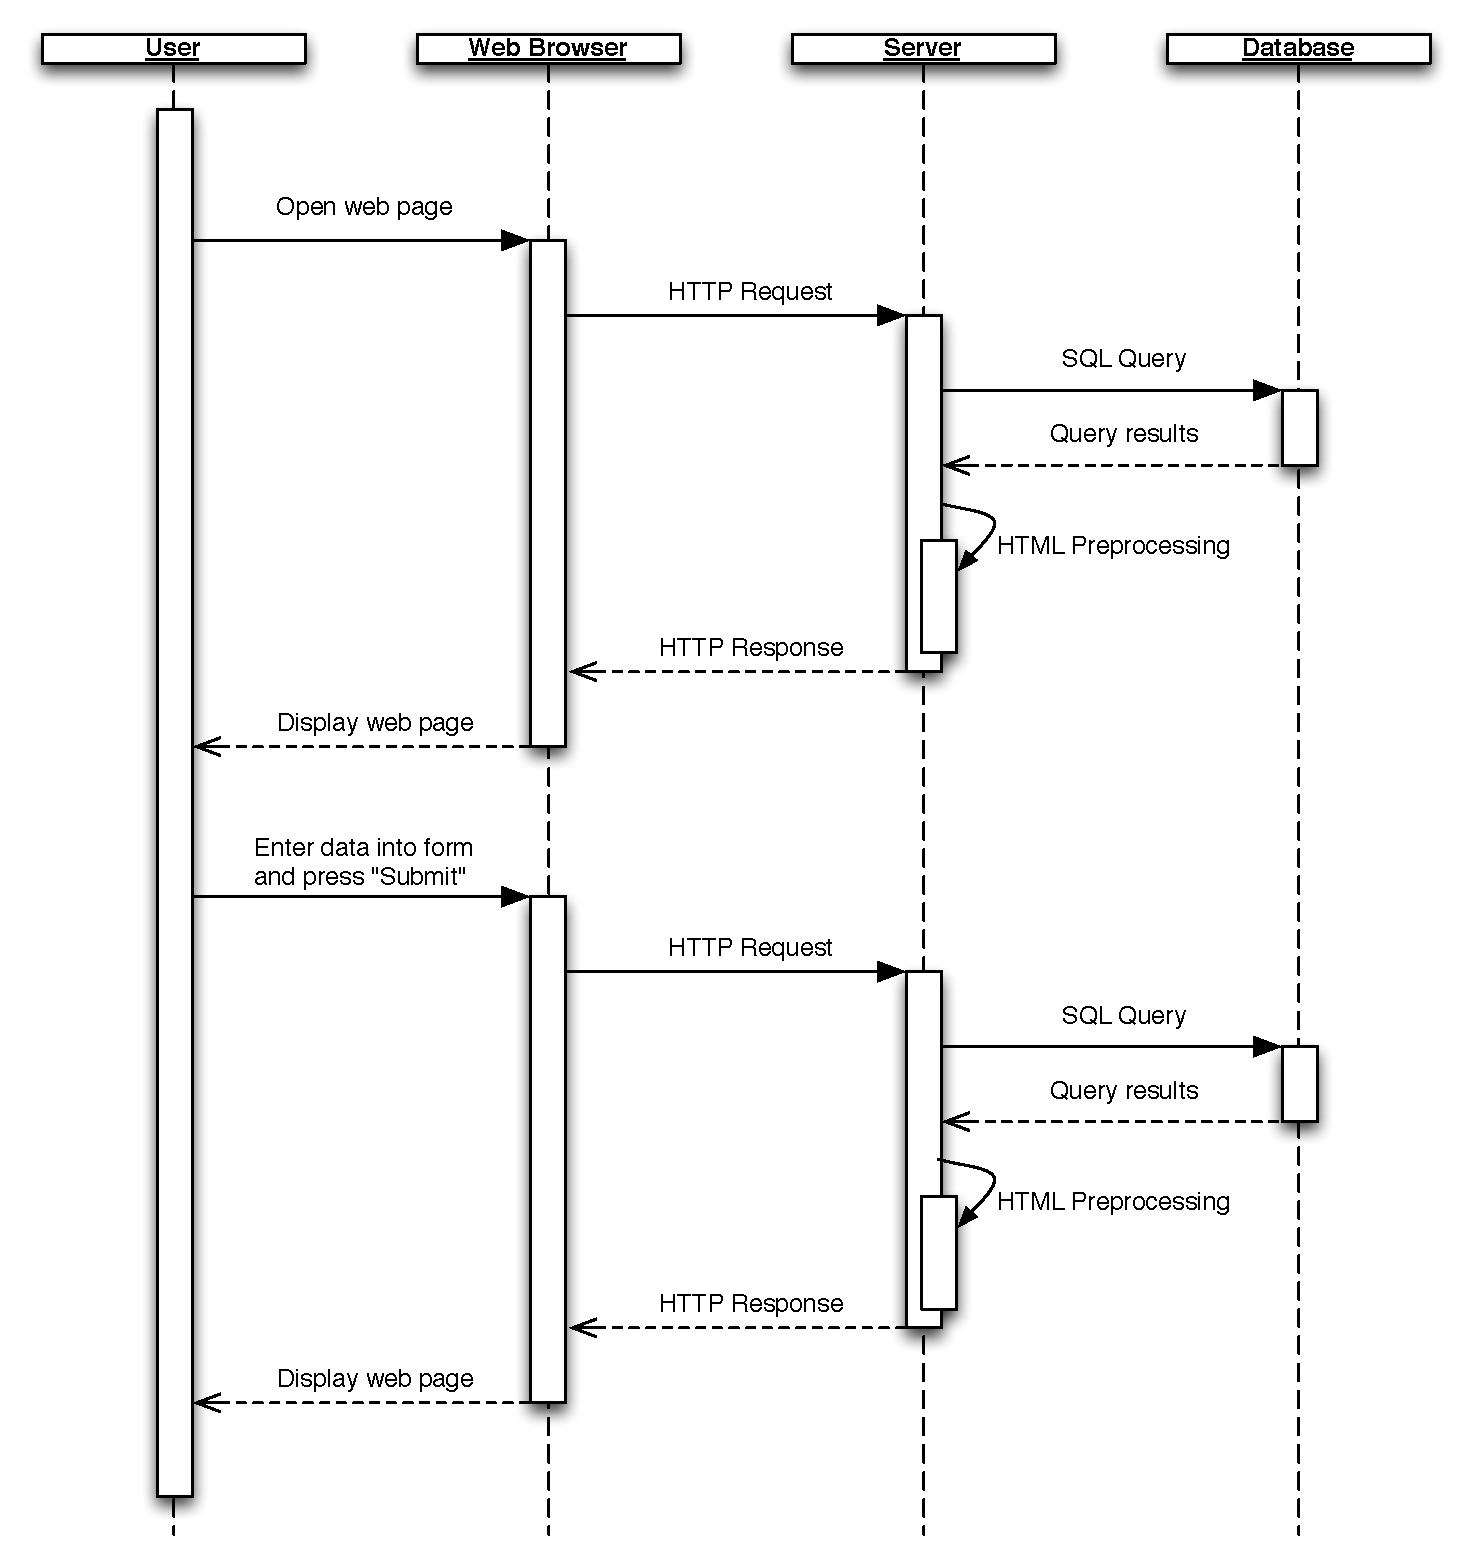
\includegraphics[width=16cm]{images/seqthinclient.pdf}
	\caption{Sequence diagram of a Thin Client user interaction}
	\label{fig:seqthinclient}
\end{figure}

An illustrating example for a Thin Client / Rich Server model are the two variants of \acl{mvc} in \ac{jsp}--based web applications, called \emph{Model 1} and \emph{Model 2}. As described by \citeasnoun[pp. 444--446]{johnson}, Model 1 provides individual \ac{jsp} pages for every section of the web application, mapping those pages to \acp{ejb}. The flow of navigation is directed by links to the different JSPs, which act as both Controller and View. The JavaBeans are the respective Models.

\begin{figure}[H]
	\centering
	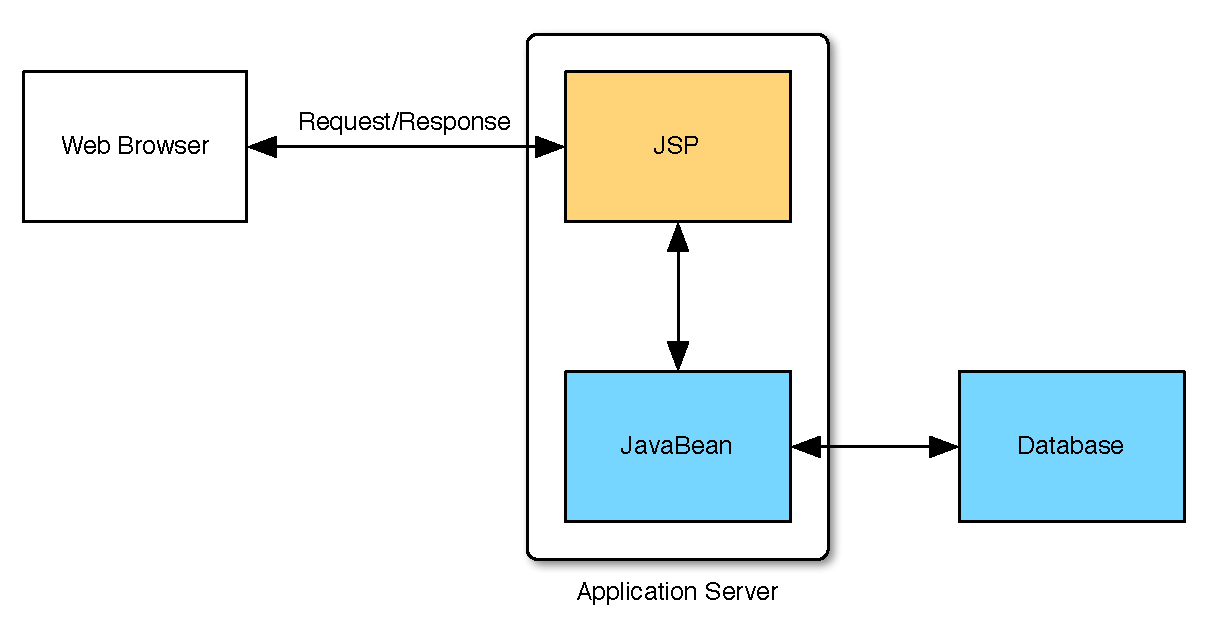
\includegraphics[width=14cm]{images/model1.pdf}
	\caption{JSP Model 1 Architecture}
	\label{fig:model1}
\end{figure}

In Model 2\label{term:model2}, the Controller part is encorporated by one central Servlet acting as an entry point into the application \cite[pp. 446 f.]{johnson}. It handles all browser requests and manages the application state. Depending on the request and the state, it selects a View (\ac{jsp}) to serve back to the browser. Similar to Model 1, the View communicates with the Model (JavaBean), but the JavaBean is modified by the Servlet instead of the \ac{jsp}. Having only one Controller differs from the \mbox{Smalltalk-80} definition of \ac{mvc}, but can be seen in some interpretations as an \emph{application controller}.

\begin{figure}[H]
	\centering
	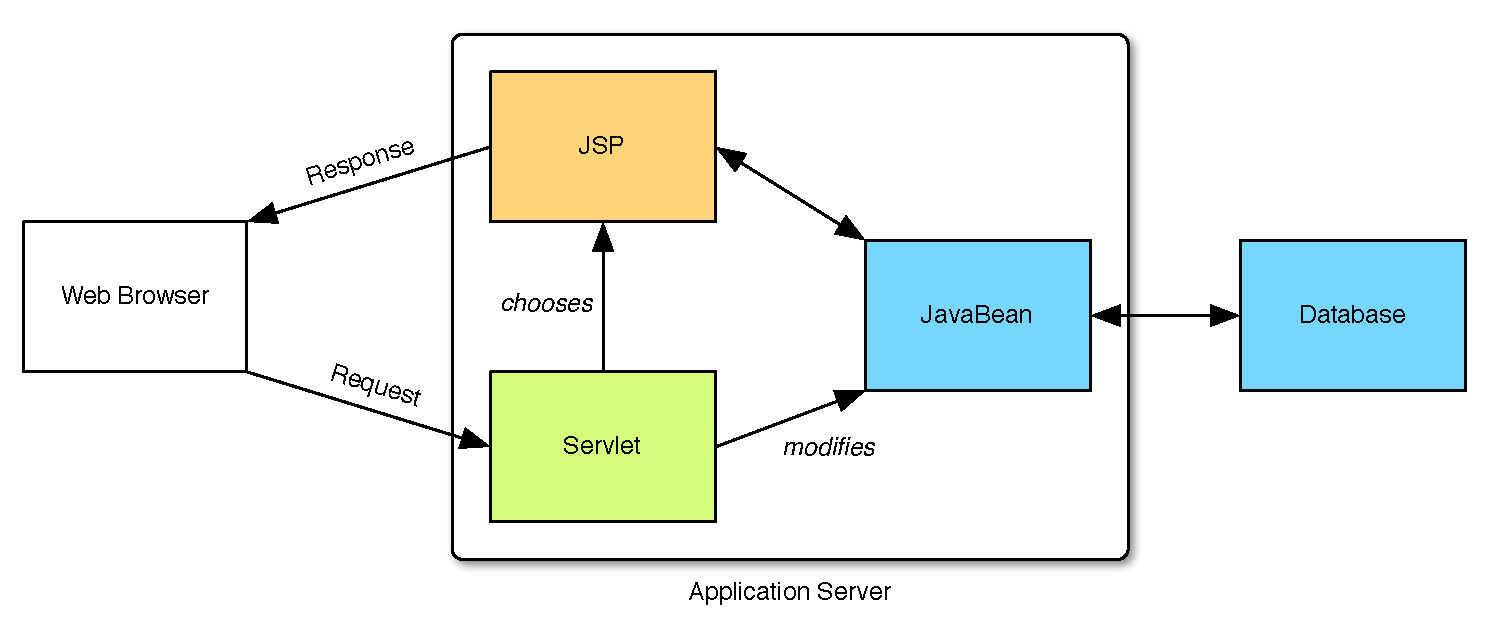
\includegraphics[width=16cm]{images/model2.pdf}
	\caption{JSP Model 2 Architecture}
	\label{fig:model2}
\end{figure}

\subsection{Rich Client}
% Ein Fat Client ist neben der Ein- und Ausgabe auch für die Verarbeitung der Daten zuständig. Lediglich zur Kommunikation und Datenspeicherung werden Dienste eines Servers genutzt. % wikipedia
From the user perspective, the key difference to a Thin Client is that the Rich Client acts \emph{like a desktop application rather than a website}.

From a business logic perspective, a Rich Client web application runs as much application logic as possible on the client side. This means, data transformation (like sorting, filtering, conversion) and referencing happens on the client side, as well as changes to the data (which then are made persistent on the server side). There still are parts that have to be executed on the server, for example security (authentication, authorisation) and the connection to a third tier (such as a database).

From a technology perspective, a Rich Client makes extensive use of JavaScript and the \ac{ajax} technique.
%This does not mean that a Thin Client has to run without JavaScript and asynchronous calls, it just means that a Rich Client leverages the power of JavaScript.
This can, for example, happen through the use of a client-side MVC pattern that has not only the View, but also the Model and the Controller running in the browser. In modern scenarios, another example is the use of Web Sockets that lets the server-side Model notify the web browser when changes happen. The key point is to reduce communication with the server to a minimum.

Figure~\ref{fig:seqrichclient} shows a sequence diagram of a user interaction with a Rich Client / Thin Server. The same activities as in Figure~\ref{fig:seqthinclient} are executed, but due to the asynchronousness of \ac{ajax} calls, the browser and user can still interact during the second request. As indicated, the web page gets only preprocessed once (when first requested). After the form submit, the processing of the returned, updated data happens in the browser, and not on the server as in Figure~\ref{fig:seqthinclient}.

Also, business logic such as input verification is executed on the client-side already (before the form is submitted). However, to ensure data consistency and security, in most implementations the submitted data --- as well as the user's authorization --- is verified on the server again.

In extremely client-sided web applications, such as \ac{ibm} \nexus, there happens no preprocessing on the server at all. On first request, the server only sends one single, nearly empty \ac{html} skeleton file. The client loads all needed functionality (mostly Dojo and \ac{idx}) via \ac{ajax}, building the \ac{gui} solely using JavaScript. There are no more ``pages'' in the sense of web pages; navigation is done using JavaScript. If the user navigates to a different application pane, \nexus\ swaps out the respective \ac{dom} nodes, which gives the feel of a real desktop application. \nexus\ is further discussed in Chapter~\ref{chap:nexus}.

This navigational pattern is described by \citeasnoun[pp. 104 f.]{osmani} with one main characteristic: the state of the application is managed on the client side, using a component that has the role of a ``router''. In Thin Client applications, the state is managed on the server side using sessions\footnote{A \gls{session} identifies interrelated requests using a session ID (usually a unique combination of alphanumeric characters) to provide state on top of the stateless \ac{http} protocol.}.

\begin{figure}[H]
	\centering
	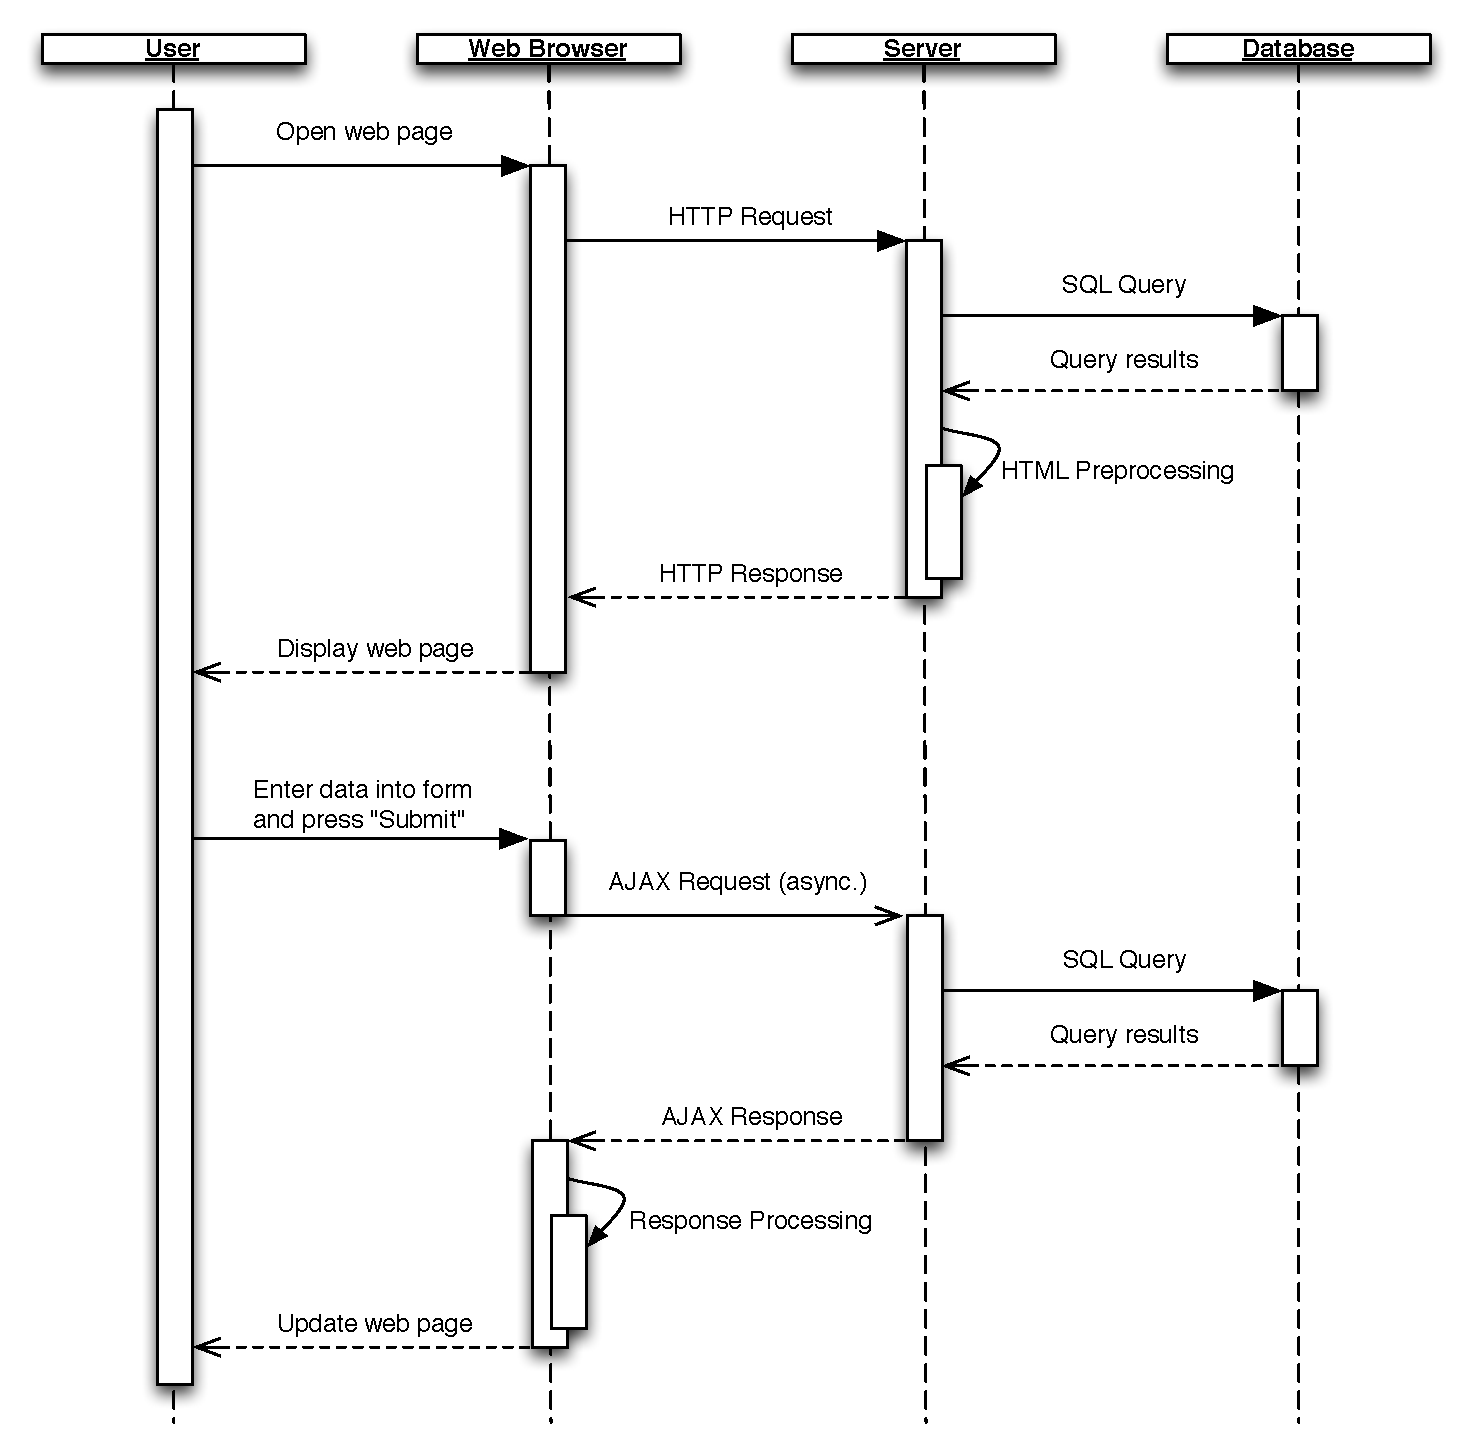
\includegraphics[width=16cm]{images/seqrichclient.pdf}
	\caption{Sequence diagram of a Rich Client user interaction}
	\label{fig:seqrichclient}
\end{figure}
